\documentclass[12pt]{article}
 
\usepackage[margin=.95in]{geometry} 
\usepackage{amsmath,amsthm,amssymb, graphicx, multicol, array}
 
\newcommand{\N}{\mathbb{N}}
\newcommand{\Z}{\mathbb{Z}}
 

\begin{document}
 
\title{SDS383C Final Project Report \\ \textbf{Inferring Causal Impact Using Bayesian Structural Time-series Models}} 
\author{Brodersen, K., Gallusser, F., Koehler, J., Remy, N., Scott, S.\\Reproduced by Juliette Franqueville
}
\maketitle

\begin{abstract}
    The abstract
\end{abstract}

\section{Introduction}
\subsection{Problem Statement}
The paper I chose  presents a Bayesian methodology for inferring causal impact of market interventions on a metric of interest. A market intervention may be the launch of an advertising campaign, the release of a new product, a feature change in a product, or others. It is desirable for companies to understand whether a market intervention has a positive effect on a given metric, such as number of sales, revenue generated, number of users acquired, etc. 

The causal impact of a treatment is defined as the difference between the observed metric (i.e. sales, number of users acquired, etc) and the metric that would have been observed had no treatment been introduced. This paper deals with time series, so the causal impact is the difference between the observed time series (i.e. sales, number of users acquired as a function of time) and the time series that would have been observed with no market intervention. The main goals of this paper are therefore to 1) predict the time series that would have been observed with no market intervention - this is called the ``counterfactual'' and 2) compare this prediction with the observed time series, where a market intervention was conducted.  A key concept in this paper is that control time-series, such as time-series for other regions where no market intervention was introduced, can be used to predict the counterfactual.

\subsection{Previous Methods}
A typical approach for performing causal inference are ``difference-in-differences'' (DD) methods. DD models a usually based on a linear model between control in treatments groups. Figure \ref{dd} describes a simple example using data I simulated. A control group (for example, sales data from another region) time-series is  available. The treatment group undergoes a  market intervention event. We can model the treatment time series as a linear model of the control time series (in the simulation, I used $y_t = x_t + 500 + \varepsilon_t$, where $y_t$ and $x_t$ are the treatment and control data points at time $t$, respectively.). Using the linear relationship inferred from pre-market intervention data and the post-intervention control group data, the counterfactual treatment time-series can be predicted. The causal impact is then the difference between the observed treatment and predicted treatment time-series post market intervention. 

\begin{figure}[!h]
    \centering
    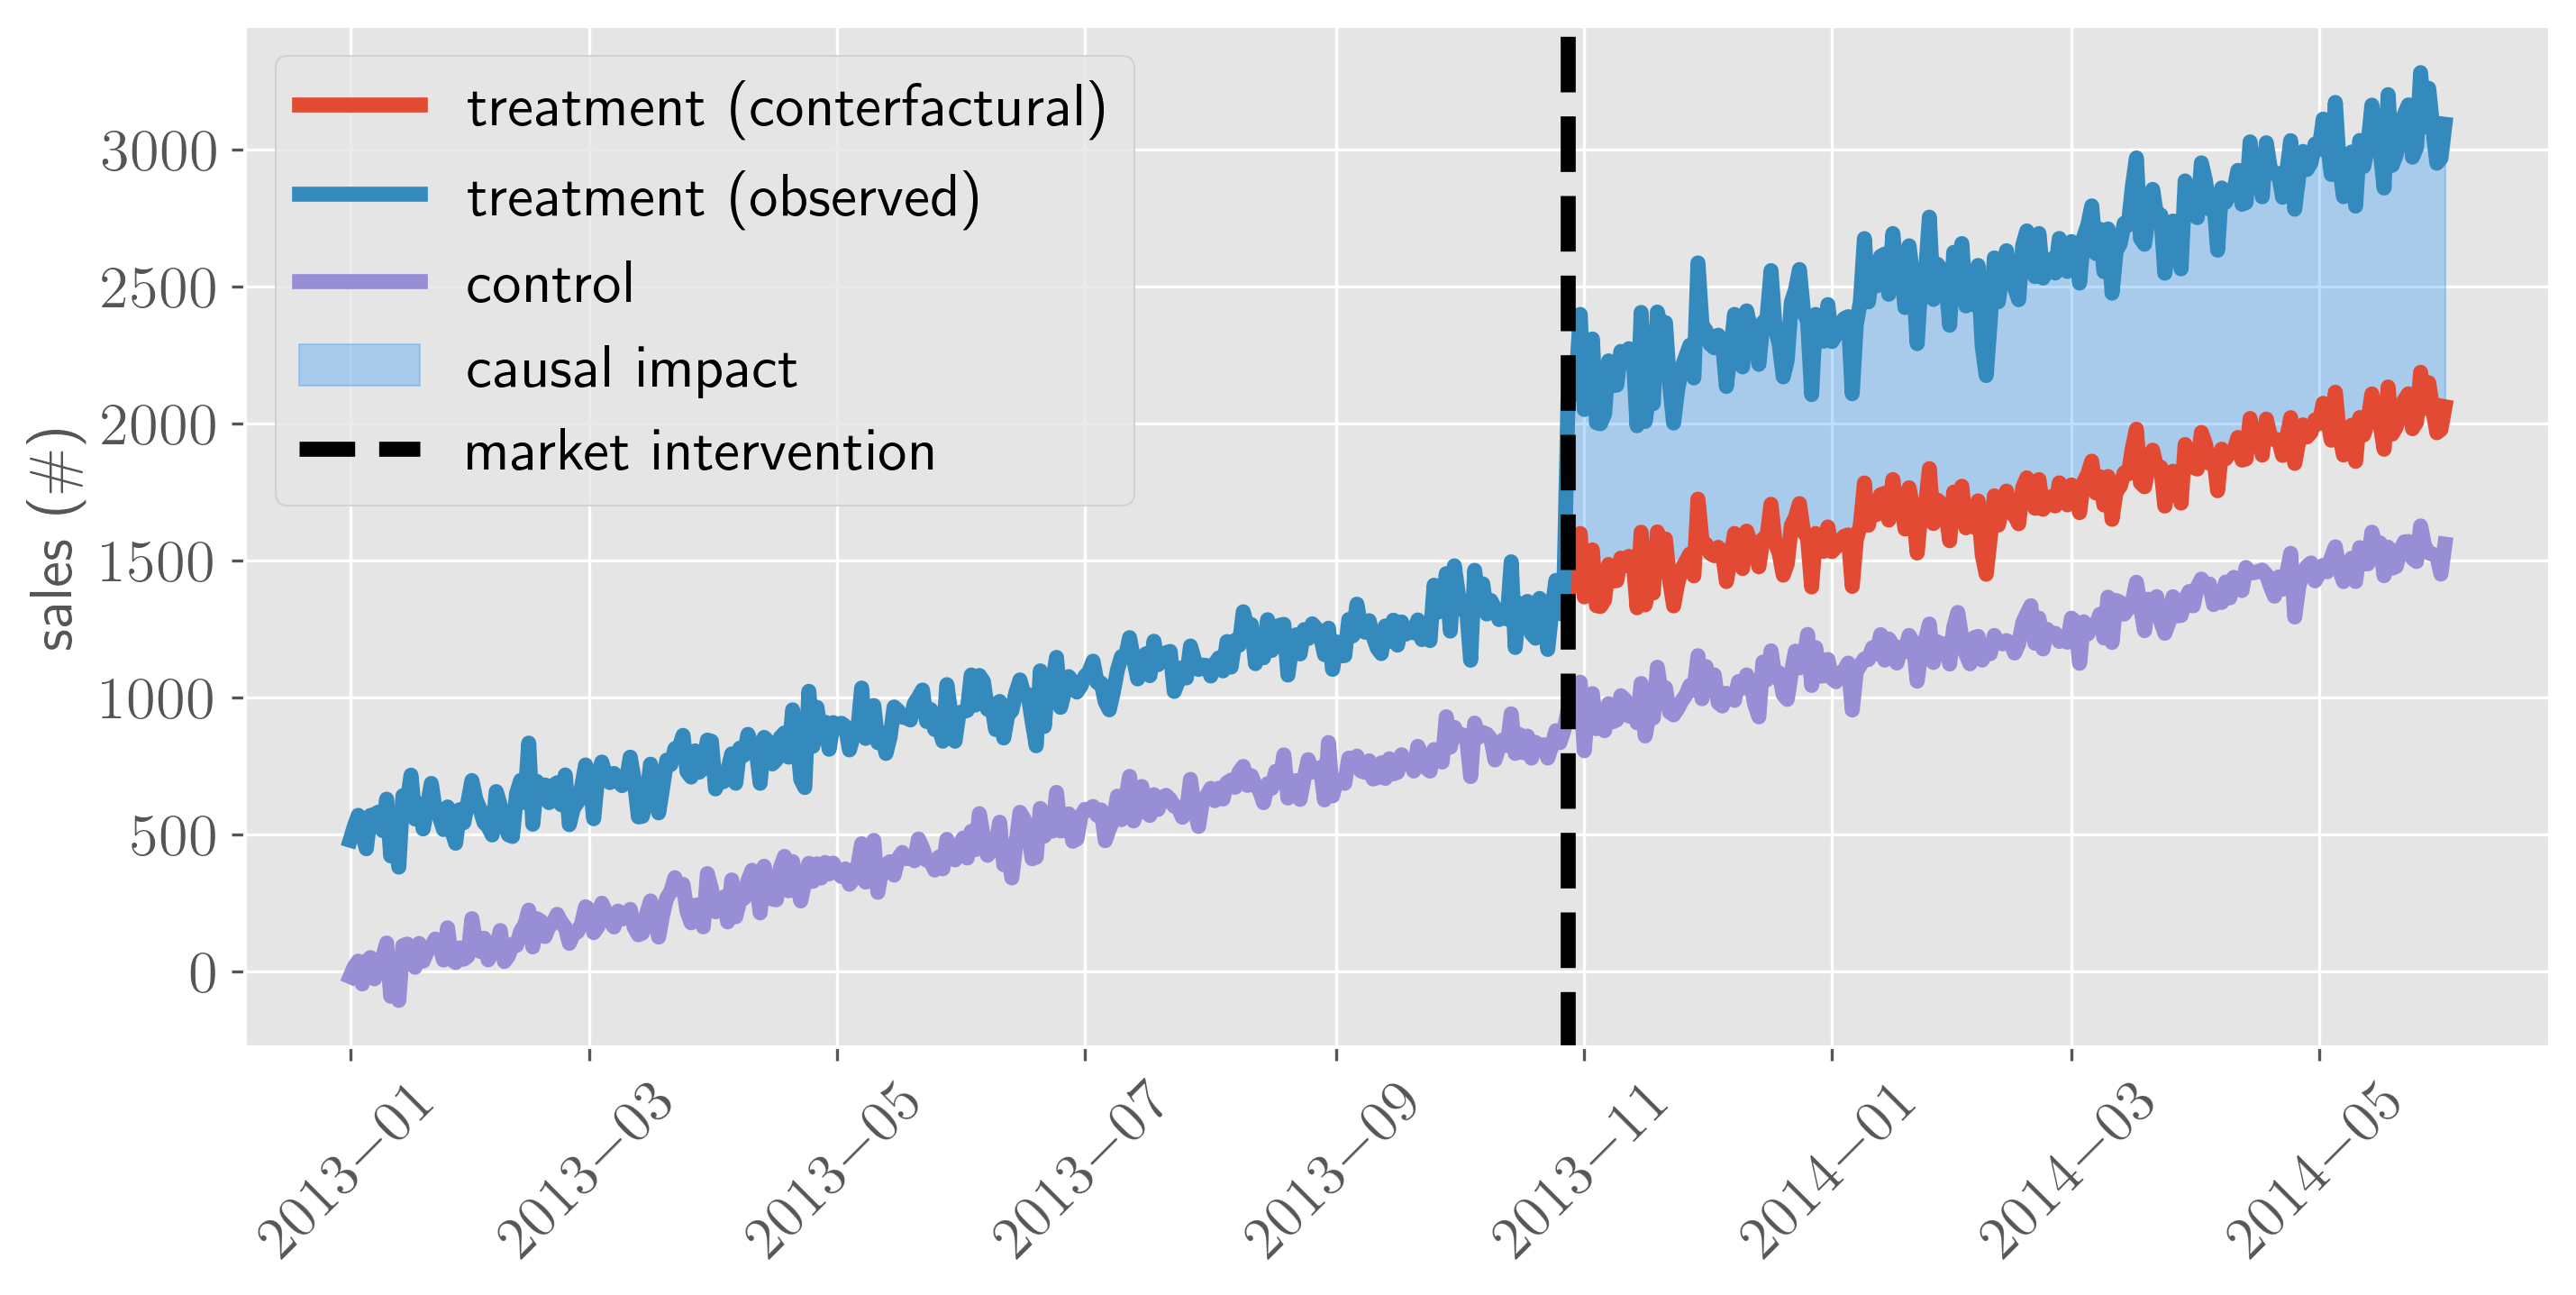
\includegraphics[scale=.6
    ]{../figures/dd.png}
    \caption{Illustration of a DD approach for inferring causal inference. }
    \label{dd}
\end{figure}

There are several limitations associated with this type of approach that this paper seeks to address. For example, DD models are generally not very flexible. Regression coefficients are usually static, which may not be a suitable assumption if they are evolving in time. The authors also wish to avoid using some of the variable selection methods that DD models use. For example, Lasso regression has been used for variable selection \cite{belloni2015program}, but this approach does not take uncertainty about which predictors to use and their coefficients, unlike Bayesian methods.

\subsection{Bayesian Structural Time-series models}
Bayesian Structural Time-series (BSTS) models are very flexible state-space models for time-series data. In fact, all ARIMA models can be specified in this manner. BSTS models can also account for dynamic regression coefficients. A BSTS model is specified as follows:

\begin{align} 
y_t &= Z_t^T\alpha_t + \varepsilon_t\\ \label{eq}
\alpha_{t+1} &= T_t \alpha_t + R_t \eta_t \label{eq1}
\end{align}
Where $\varepsilon_t \sim \mathcal{N}(0, \sigma^2)$ and 
$\eta_t \sim \mathcal{N}(0, Q_t)$. $ Q_t$ is a $p \times p$ matrix, which can be diagonal or not. The first line is the observation equation, and the second is the state equation. $y_t$ is the observed response (scalar), while $\alpha_t$ is a hidden state (scalar or vector, not observed). $Z_t$ is a $p \times n$ matrix, which can for example contain covariates for control groups or rows of 1s, depending on how the model is structured.  $T_t$ is a $p \times p$ ``transition matrix'' and $R_t$ is a $p \times p$ ``control matrix''. Both matrices are populated based on the model. Some common, simple forms of models expressed in this format are shown below. \\

\subsubsection{AR(1) Model}

An AR(1) model  can be written as a BSTS model using:

\begin{align}
    y_t &= \mu_t + \varepsilon_t \\
    \mu_{t+1} &= \phi \mu_t + \eta_t
\end{align}

Which can be re-written in the same format as equations \label{eq} and \label{eq1} by setting $\mu_t = \alpha_t$, $\mu_{t+1} = \alpha_{t+1}$, $Z_t^T = 1$, $T_t = \phi$, $R_t = 1$.


\subsubsection{Local Level}
A local level  can be written as:
\begin{align}
    y_{t} &= \mu_t + \varepsilon_t \\
    \mu_{t+1} &= \mu_t + \eta_t 
    \end{align}

Which can be re-written in the same format as equations \label{eq} and \label{eq1} by setting $\mu_t = \alpha_t$, $\mu_{t+1} = \alpha_{t+1}$, $Z_t^T = 1$, $T_t = 1$, $R_t = 1$.

\subsubsection{Linear Regression (Static Coefficients)}\label{linreg}
A linear regression can be written as:

\begin{align}
    y_{t} &= x_t\beta + \varepsilon_t\\
\end{align}

Which can be re-written in the same format as equations \label{eq} and \label{eq1} by setting $\alpha_t=1$,  $Z_t^T = x_t\beta$.

\subsubsection{Linear Regression (Dynamic Coefficients)}
A linear regression with dynamic coefficients can be written as:

\begin{align}
    y_{t} &= x_t\beta_t + \varepsilon_t\\
    \beta_{t+1} &= \beta_t + \eta_t
\end{align}

Which can be re-written in the same format as equations \label{eq} and \label{eq1} by setting $\beta_t = \alpha_t$, $\beta_{t+1}=\alpha_{t+1}$, $Z_t^T = x_t$, $T_t = 1$, $R_t = 1$.\\

Other state-space models not explicitly  listed include seasonal models, local linear trends, semi-local linear trends, etc. To allow for more flexibility, state components can be assembled by concatenating their observation and hidden state vectors $Z_t$ and $\alpha_t$ and re-arranging other matrices ($R_t, T_t$) as elements in block diagonal matrices. A concrete example showing how to assemble different models is shown in section \ref{toy}.




\section{Methods}
\subsection{Spike-and-Slab Priors}
The paper uses spike-and-slab priors for static regression coefficients (that is, coefficients in \ref{linreg}). Specifying spike-and-slab priors over regression coefficients is essentially a Bayesian method for variable selection, which involves keeping only necessary covariates in the model. Lasso is a typical frequentist methods for variable selection in regressions. For a static regression component with multiple $\beta_i$ coefficient formulated as:

\begin{align}
    y_t &=  \boldsymbol{X}_t\boldsymbol{\beta} + \varepsilon_t\\
     \varepsilon_t &\sim \mathcal{N}(0, \sigma^2)
\end{align}

A spike-and-slab prior has the form:

\begin{align}
    \beta_i \sim (1-\pi_i)\delta_0 + \pi_i\mathcal{N}(0, \tau^2\sigma^2)
\end{align}


Where $\pi_i \in [0, 1]$, and $\delta_0$ is the Dirac delta function. With $\pi_i = 0.5$, $\sigma^2 = 1$, $\tau^2 = 1$, this distribution is shown in Figure \ref{prior}



\begin{figure}[!h]
    \centering
    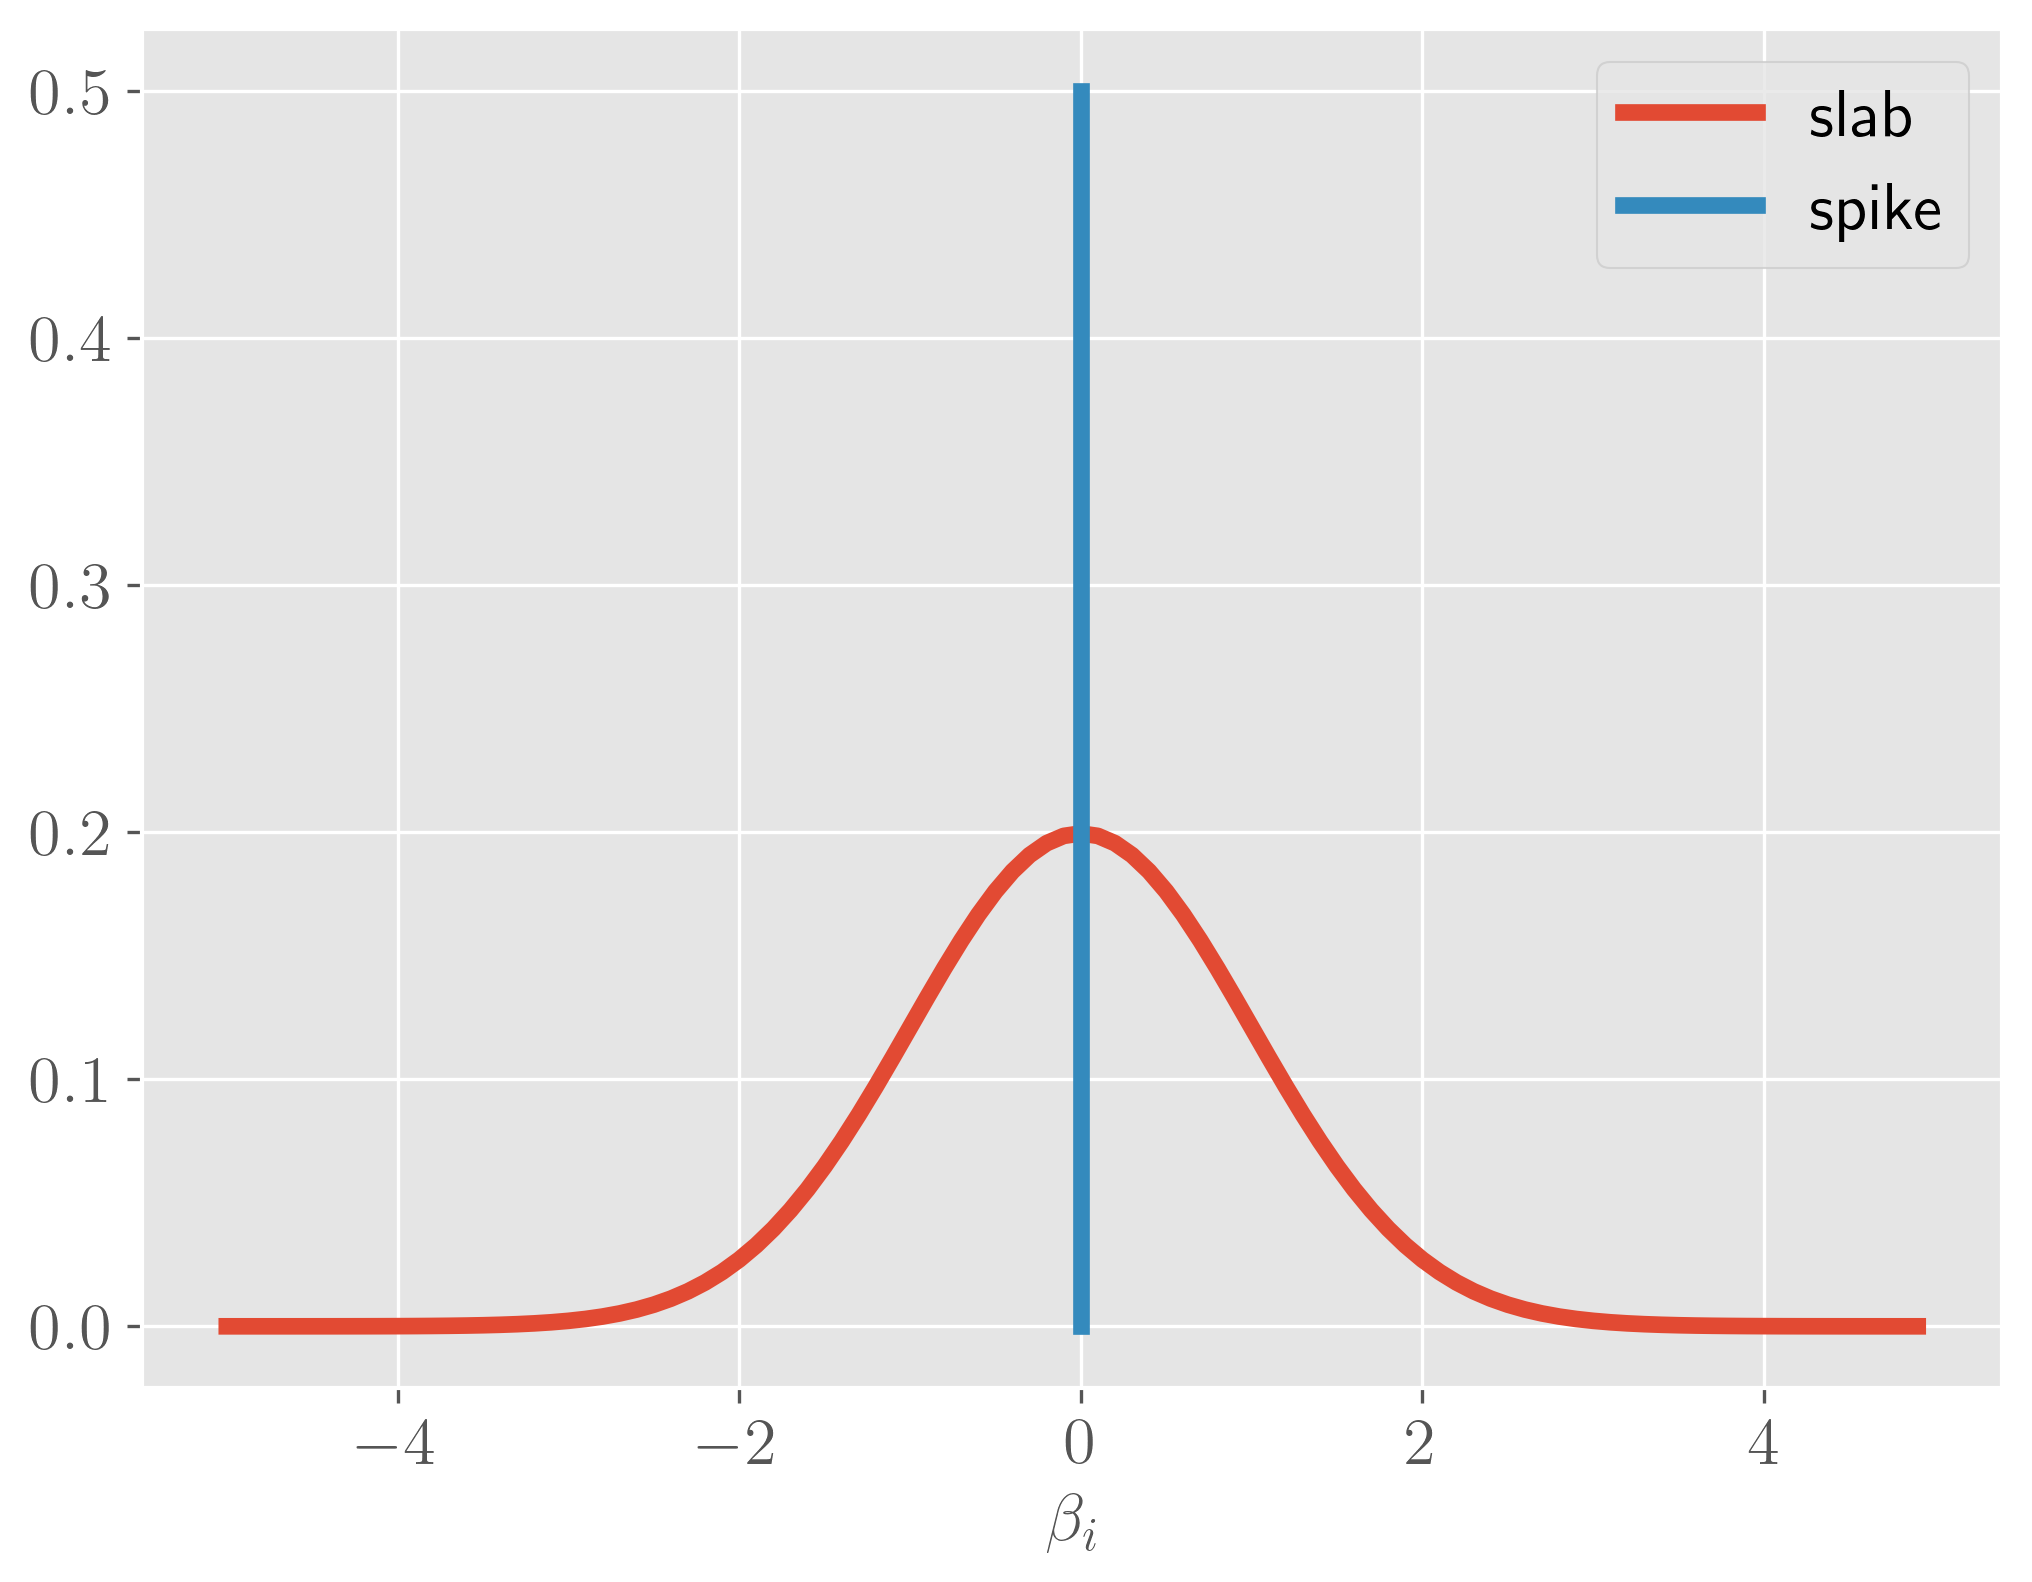
\includegraphics[scale=.6
    ]{../figures/spike.png}
    \caption{Spike-and-slab prior illustration.}
    \label{prior}
\end{figure}

I reproduced this aspect of the paper by creating a simulated dataset using:

\begin{align*}
    y_t& = x_{1, t}\beta_1 + x_{2, t}\beta_2 + \varepsilon_t\\
    \varepsilon_t &\sim \mathcal{N}(0, \sigma^2)
\end{align*}

With $\beta_1 = 10$,  $\beta_2 = 0.05$, and $\sigma^2 = 4$. Figure \ref{toydata} shows the dataset created. 

\begin{figure}[!h]
    \centering
    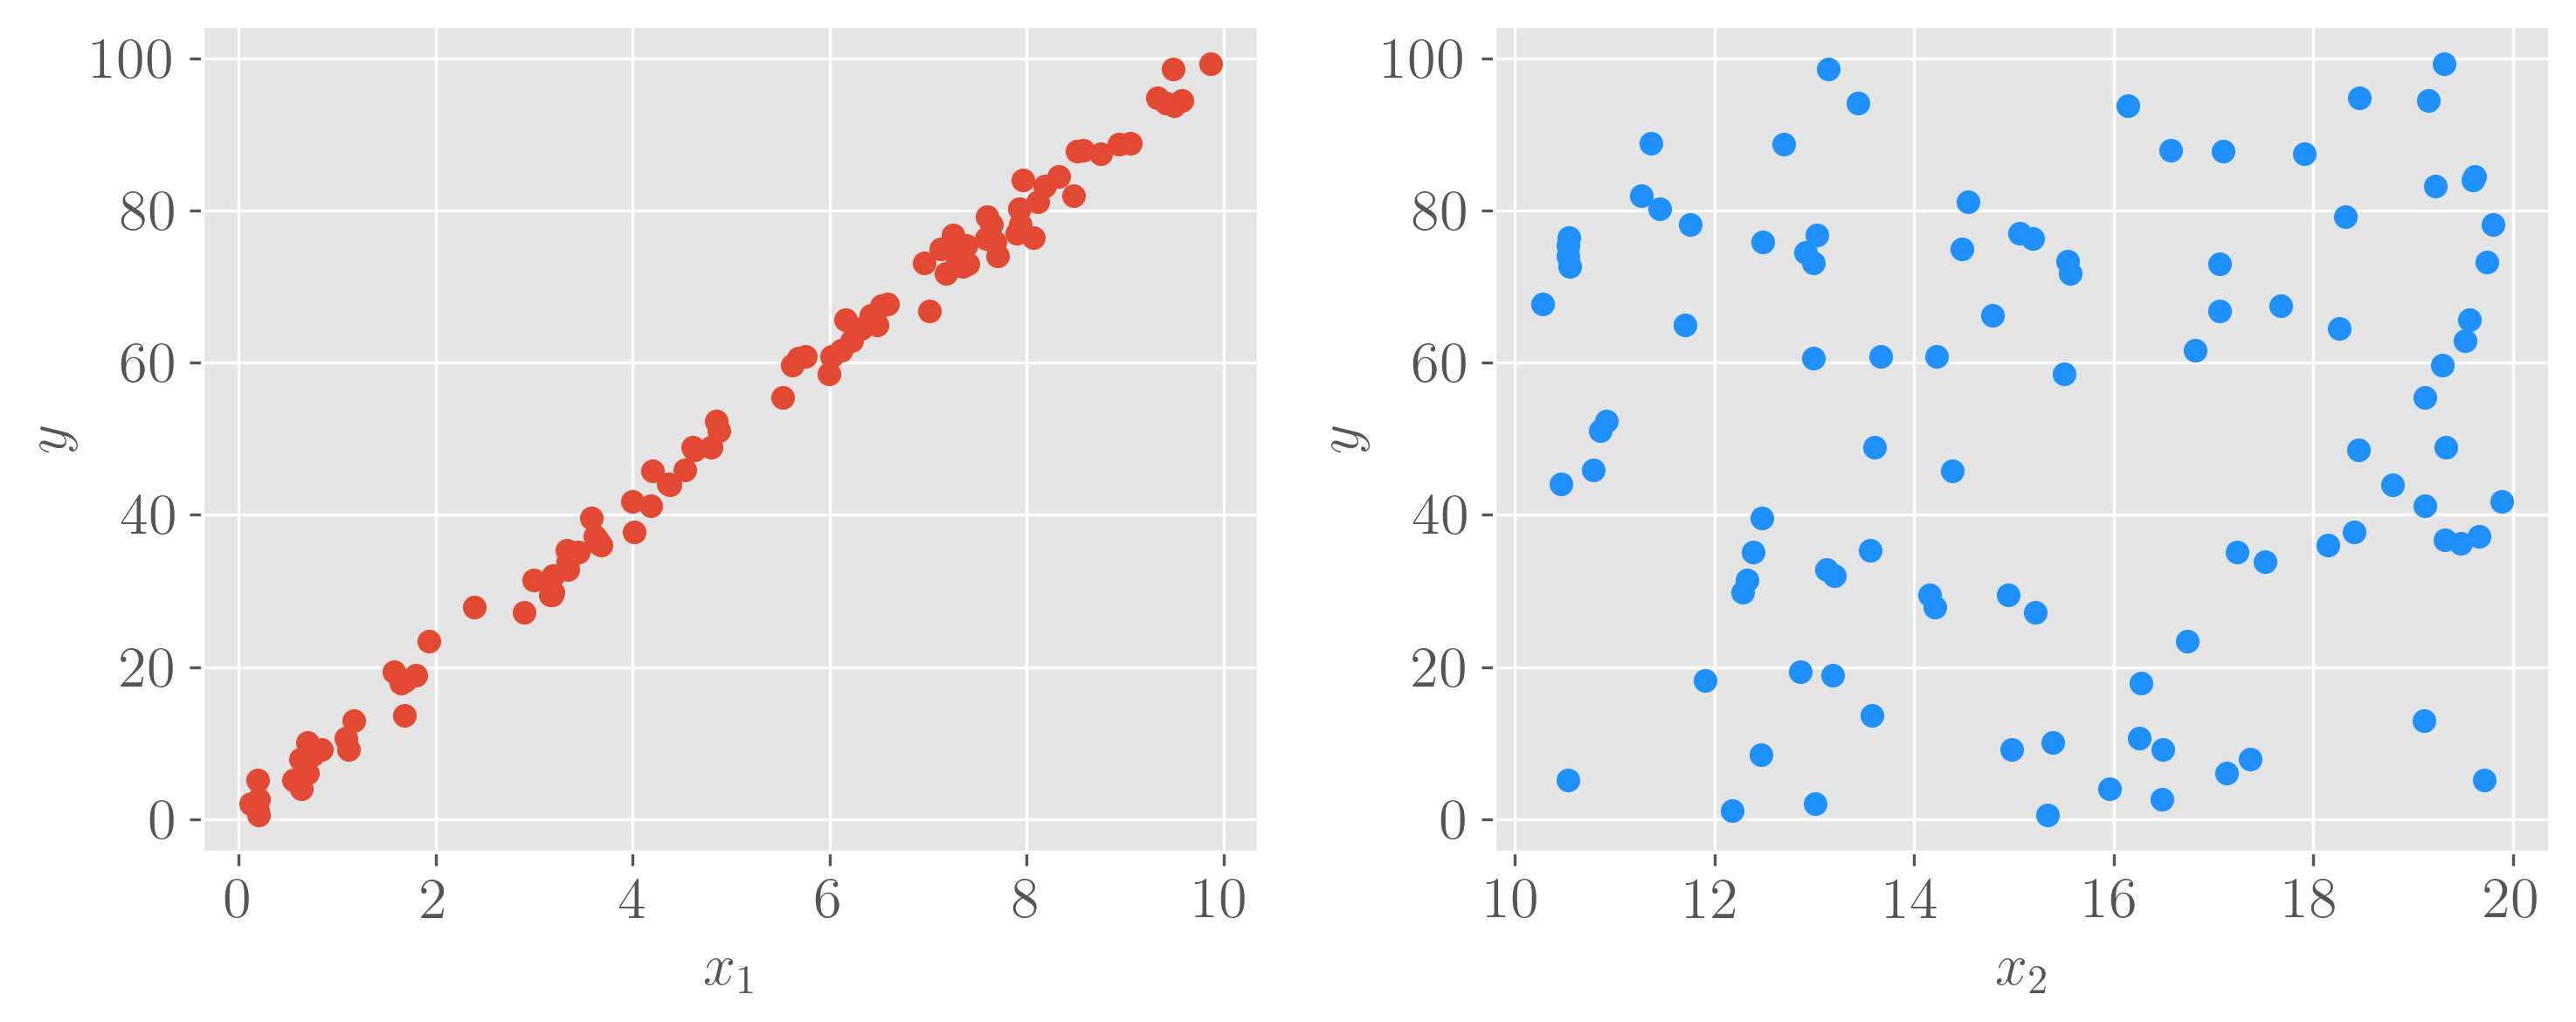
\includegraphics[scale=.6
    ]{../figures/toydata.png}
    \caption{Simulated data for reproduction of regression coefficient inference using spike-and-slab priors.}
    \label{toydata}
\end{figure}

I used the following priors:

\begin{align*}
    \tau^2 &\sim IG(1, s^2/2)\\
    \sigma^2 &\sim IG(\alpha_1, \alpha_2)\\
    \pi_i &\sim Bernoulli(\theta)\\
    \theta & \sim Beta(a, b)
\end{align*}

The conditional posteriors were (note that I checked my answers against \cite{andrade2020disjunct}):

\begin{align}
    P(\theta|\boldsymbol{\pi}) &\sim Beta(a + \sum_{i=1}^p \pi_i, b + \sum_{i=1}^p [1-\pi_i])\\
    z_i &\sim Bernoulli(\pi_i)\\
    P(\boldsymbol{\beta}|\sigma^2, \tau^2) &= \begin{cases}
     \mathcal{N}\left(\left[\boldsymbol{X}^T\boldsymbol{X} \frac{1}{\sigma^2} + \boldsymbol{I}\frac{1}{\sigma^2\tau^2}\right]^{-1}\boldsymbol{X}^T \boldsymbol{y} \frac{1}{\sigma^2}, \left[\boldsymbol{X}^T\boldsymbol{X} \frac{1}{\sigma^2} + \boldsymbol{I}\frac{1}{\sigma^2\tau^2}\right]^{-1}\right)& \text{if } z_i = 1\\
    0             & \text{if } z_i = 0
\end{cases}\\
P(\sigma^2|\boldsymbol{\beta}) &\sim IG\{\alpha_1 + n/2, \alpha_2 + \frac{1}{2}(\boldsymbol{y}-\boldsymbol{X}\boldsymbol{\beta})^T(\boldsymbol{y}-\boldsymbol{X}\boldsymbol{\beta})\} \\
P(\tau^2|\boldsymbol{\beta}, \boldsymbol{\pi}) &\sim IG(1/2 + 1/2\sum_1^{p}\pi_i, s^2/2 + \boldsymbol{\beta}^T\boldsymbol{\beta}/2\sigma^2)\\
\end{align}
And finally, $\pi_i$ is updated using 

\begin{align}
    1-\pi_i = \frac{1-\theta}{(\sigma^2\tau^2)^{-1/2}\text{exp}\left(\frac{\sum_1^n x_j(y_j - X_{-i, j}\beta_{-i, j})}{2\sigma^2(\sum_1^n x_j^2 + 1/\sigma^2)}\right)  \left(\frac{\sigma^2}{\sum_1^n x_j^2 + 1/\sigma^2}\right)^{1/2}\theta   + (1-\theta)  }
\end{align}

Where $\boldsymbol{X}_{-i}$ and $\boldsymbol{\beta}_{-i}$ are $\boldsymbol{X}$ and $\boldsymbol{\beta}$ with the column and row corresponding to $i$ removed. At each iteration, $z_i$ is drawn from a Bernoulli distribution with $\pi_i$ parameter. The figures below show the posterios for $\beta_1$ and $\beta_2$.





\subsection{Kalman Filtering and Smoothing}
\subsection{Gibbs Sampling}

\section{Example with Simulated Data}\label{toy}
\subsection{Model}


\bibliographystyle{ieeetr} 
\bibliography{ref}
\end{document}
